\documentclass[mathserif]{intbeamer}
%\usepackage{etex}
\usepackage[utf8]{inputenc}
\usepackage[english]{babel}
%\usepackage{qrcode}
%\usepackage[space]{grffile}
\usepackage{subcaption}
\captionsetup[subfigure]{skip=-5pt} % global setting for subfigure
%\usepackage{aligned-overset}
\usepackage{trfsigns}

\usepackage{../paper/macros}

%% *** Tikz, PGF and AudioIcons ***
%\usepackage{tikz, audioicons}
%\usetikzlibrary{calc,%
%  decorations.pathreplacing,%
  % decorations.markings,%
  % calc,%
  % arrows,%
  % through,%
  % intersections,%
  % positioning}

%\definecolor{activecolor}{RGB}{255, 0, 0}
% \definecolor{loudspeakercircle}{RGB}{236, 236, 236}
% \definecolor{focuscircle}{RGB}{254, 204, 0}
% \definecolor{darkgreen}{rgb}{0,0.5,0}
% \definecolor{orange}{rgb}{1.0,0.5,0}
% \definecolor{mauve}{RGB}{224,176,255}
% \definecolor{teal}{RGB}{64,224,208}

% \makeatletter
% \tikzset{
%   dot diameter/.store in=\dot@diameter,
%   dot diameter=3pt,
%   dot spacing/.store in=\dot@spacing,
%   dot spacing=10pt,
%   dots/.style={
%     line width=\dot@diameter,
%     line cap=round,
%     dash pattern=on 0pt off \dot@spacing
%   }
% }
% \makeatother

%% *** Importing Stuff ***
%\usepackage{import}

%% *** Mathsymbols ***
%\usepackage{soundfield}
%\sfrenewsymbol{cylm}{\mu}

%\usepackage{nicefrac}
%\DeclareFontFamily{U}{wncy}{}
%\DeclareFontShape{U}{wncy}{m}{n}{<->wncyr10}{}
%\DeclareSymbolFont{mcy}{U}{wncy}{m}{n}
%\DeclareMathSymbol{\Sha}{\mathord}{mcy}{"58}

%% *** Additional Commands extending Beamer ***
%\newcommand{\itemplus}[1][+]{\item[\textcolor{darkgreen}{\textbf{#1}}]}
%\newcommand{\itemminus}[1][--]{\item[\textcolor{red}{\textbf{#1}}]}
%\newcommand{\itemattent}[1][!\,]{\item[\textcolor{orange}{\textbf{#1}}]}
%\newcommand{\itemcheck}{\itemplus[$\checkmark$]}
%\newcommand{\itemcross}{\itemminus[$\boldsymbol{\times}$]}

%\newenvironment{itemizeblock}[1]{ %
%  \begin{block}{#1} %
%    \begin{itemize} %
%    } %
%    { %
%    \end{itemize} %
%  \end{block} %
%} %

% ===== titlepage info =====
\title[Audibility Constant Phase Shifts]%
  {Detection of Constant Phase Shifts in\\Filters for Sound Field Synthesis}

\author[Schultz et al.]{%
    \underline{Frank Schultz},
    Nara Hahn,
    Sascha Spors
}

\date[2019-09-28]{%
  5th ICSA, Ilmenau, ORAL-5-3\\
}

\institute[]{Institute of Communications Engineering, University of Rostock}

% ===== remove total number of slides from pagenumber =====
\setbeamertemplate{page number in head/foot}[nototal]
\setbeamersize{text margin left=\logomargin}
\setbeamertemplate{blocks}[rounded]
\setbeamercolor{block title}{fg=rostock-uni, bg=white}

\begin{document}
\maketitle
%
%
%
\begin{frame}{Introduction}
\begin{figure}
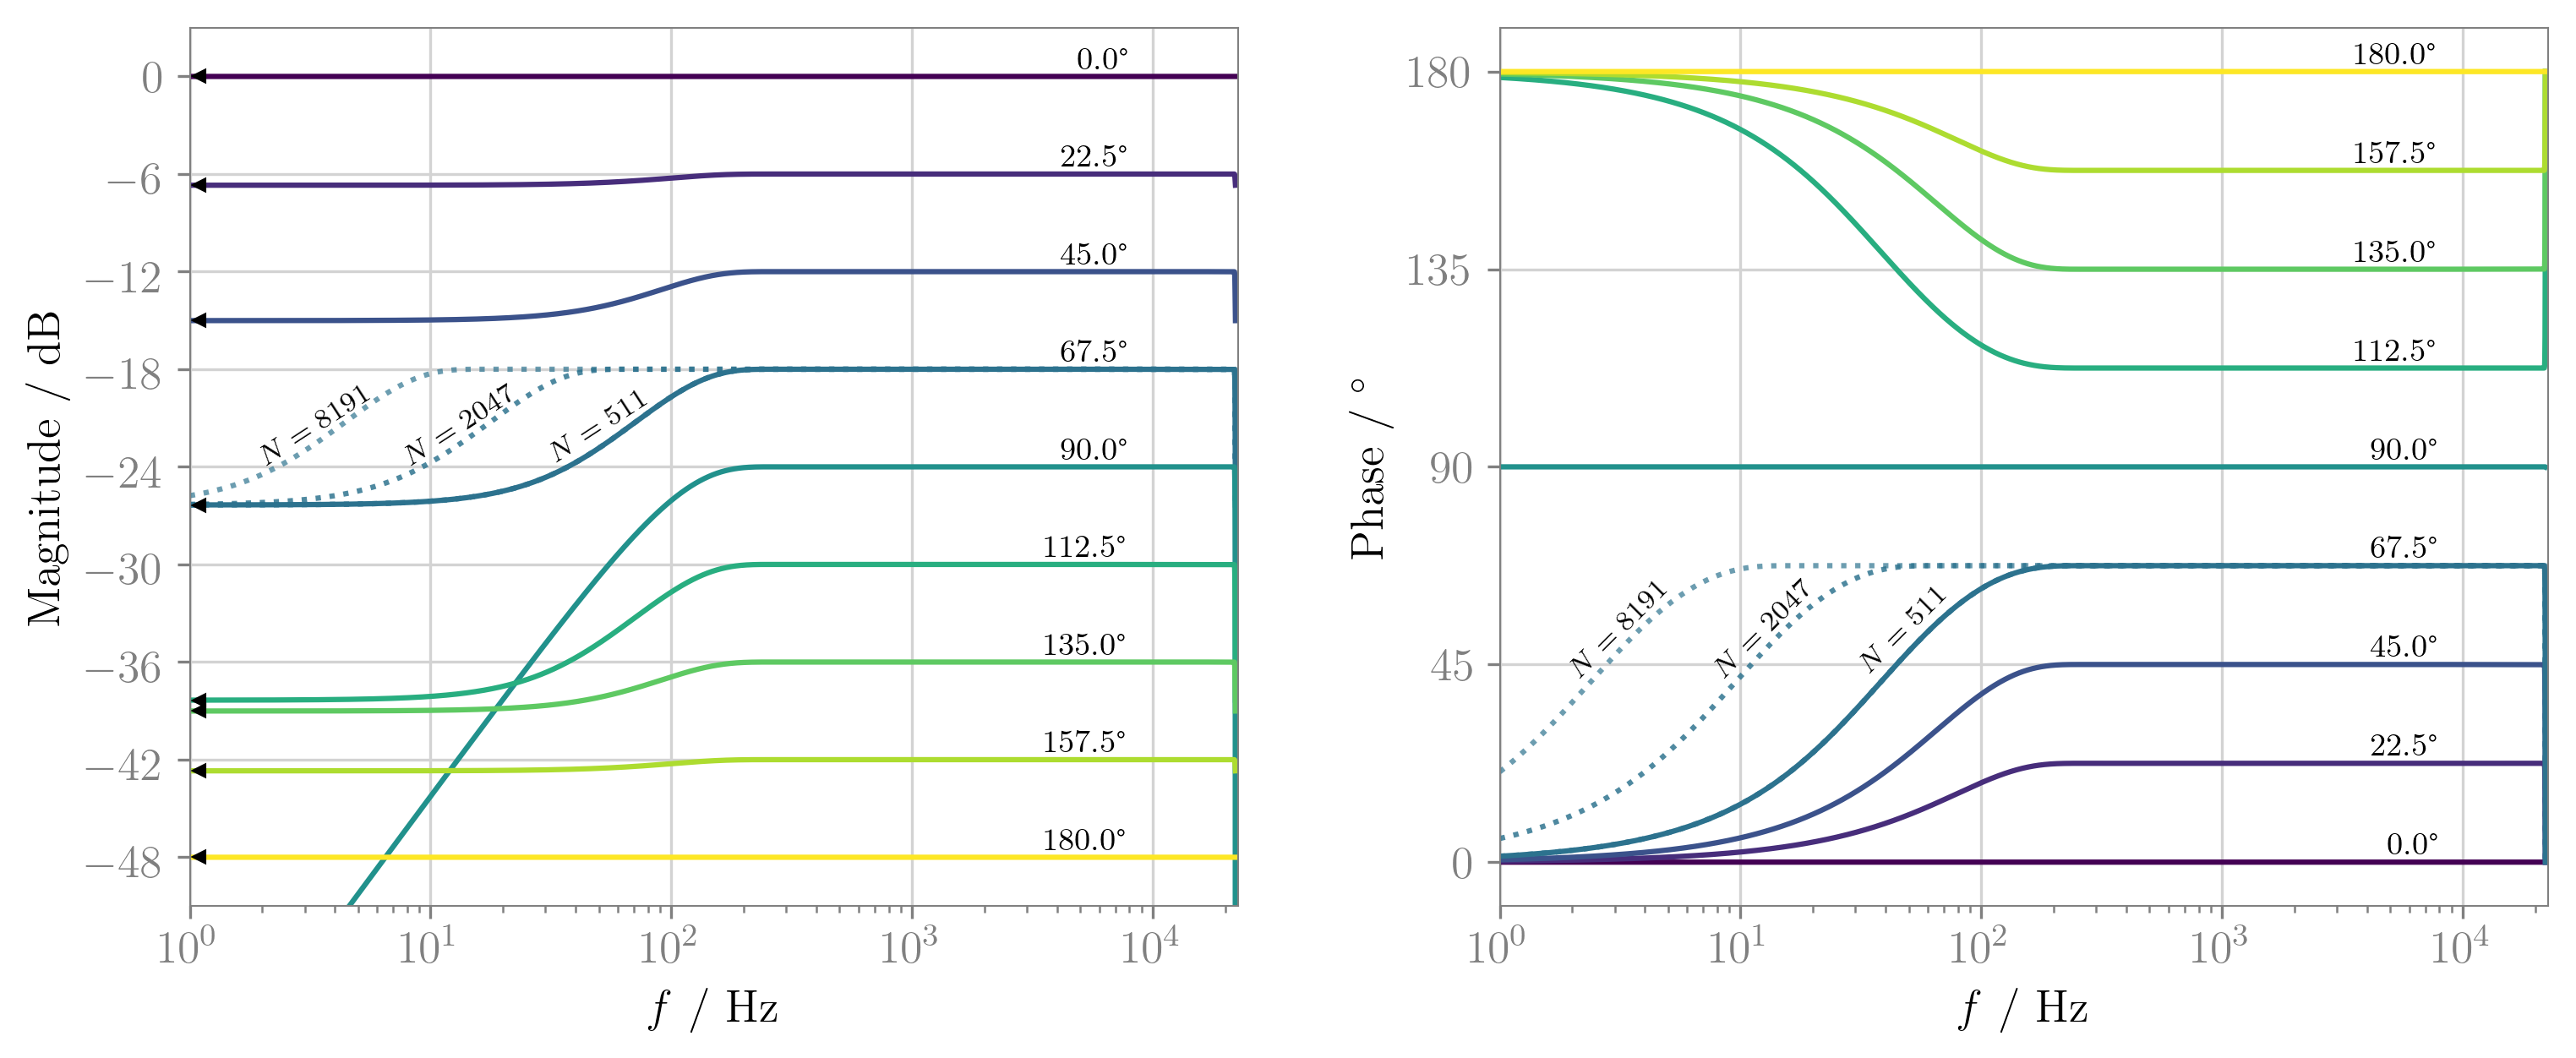
\includegraphics[width=\textwidth]{../paper/graphics/spectra_filterorder510}
\end{figure}
simple signal flow diagram, SFS filter

\begin{itemize}
\item  technical issues
\item perceptual issues
\end{itemize}
\end{frame}
%
%
%
\begin{frame}{Sound Field Synthesis Filter}
equations and sketches for 3D, 2.5D WFS
\end{frame}
%
%
%
\begin{frame}{Types of Phase Distortion}
min phase

max Phase

linear Phase

zero group delay

constant phase

audibility / perceptibilty of phase / group delay distoritions
important studies

\end{frame}
%
%
%
\begin{frame}{Example: Constant Phase Shifts of Castanets}
\begin{figure}
\includegraphics[width=\textwidth]{../notebooks/phase-shifted-signals-and-envelope}
\end{figure}
\end{frame}
%
%
%
\begin{frame}{Crest Factor}
\begin{figure}
\includegraphics[width=\textwidth]{../paper/graphics/crest-factor-and-square-waves}
\end{figure}
\end{frame}
%
%
%
\begin{frame}{Constant Phase Shift = Fractional Hilbert Transform}
\begin{align}
H(e^{i\Omega}) &=
\begin{cases}
e^{+i\varphi}, & 0 < \Omega < \pi\\
e^{-i\varphi}, & -\pi < \Omega < 0\\
\cos\varphi, & \Omega = 0, \pi
\end{cases}
\label{eq:def-dtft}
\end{align}
\begin{align}
H(e^{i\Omega})
= \cos\varphi
- \sin\varphi\cdot\Hh(e^{i\Omega}),
\label{eq:decomp-dtft}
\end{align}
with
$\Hh(e^{i\Omega})\coloneqq-i\cdot\sgn{\Omega}$ denoting
the transfer function of the Hilbert transformer
\begin{figure}
\includegraphics[width=\textwidth]{../paper/graphics/discrete-ir-phi-45}
\end{figure}
\end{frame}
%
%
%
\begin{frame}{Constant Phase Shift for Aperiodic Signals}
skectch for convolution of infinite with finite signals
windowing problem

listening examples hotel, pink noise

\end{frame}
%
%
%
\begin{frame}{Constant Phase Shifts for Periodic Signals}
skectch DFT frames superosition

listening examples square, castanets

\end{frame}
%
%
%
\begin{frame}{Listening Experiment}

Is constant phase shift audible?


Hypothesis

ABX Test Design Considerations

Post Hoic CHi

\end{frame}
%
%
%
\begin{frame}{Listening Experiment Org}
VP, age, time

\end{frame}
%
%
%
\begin{frame}{Listening Experiment Results}
\begin{figure}
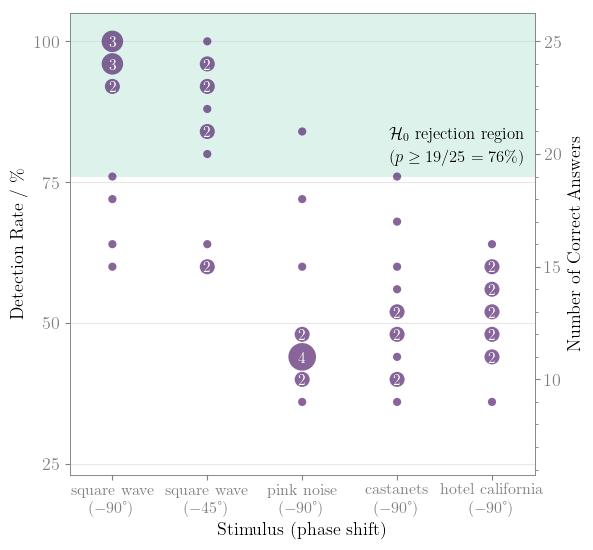
\includegraphics[width=0.67\textwidth]{../paper/graphics/scatter}
\end{figure}
\end{frame}
%
%
%
\begin{frame}{Conclusion}
\end{frame}
%
%
%



\end{document}
